\documentclass[dissertation]{softeng}

\usepackage{times}
\usepackage[utf8]{inputenc}

\usepackage[backend=biber,
            hyperref=false,
            natbib=true,
            citestyle=authoryear,
            bibstyle=authoryear-comp,
            url=false,
            isbn=false,
            doi=false,
            dashed=false,
            maxcitenames = 2, 
            mincitenames = 1, 
            maxbibnames = 3,
            firstinits = true,
            labelyear=true,  
            uniquename=false, 
            uniquelist=false,
            terseinits = false]{biblatex}

\addbibresource{mydissertation.bib}

\title{Extending BDD\\A systematic approach to handling non-functional requirements}
\author{Pedro Moreira}
\college{Kellogg College}
\organisation{University of Oxford}
\award{Software Engineering}

\usepackage[english, status=draft]{fixme}
\fxusetheme{color}

\usepackage{xspace}
\newcommand{\nfrs}{non-functional requirements\xspace}
\newcommand{\Nfrs}{Non-functional requirements\xspace}

\usepackage[english]{babel}
\usepackage[autostyle=true,english=british]{csquotes}
\SetCiteCommand{\citep}


\usepackage{pgfplotstable}
\usepackage{booktabs}
\usepackage{array}
\usepackage{colortbl}
\usepackage{tabularx}
\usepackage{graphicx} %package to manage images
\graphicspath{ {Images/} }

\colorlet{tableheadcolor}{gray!25} % Table header colour = 25% gray
\newcommand{\headcol}{\rowcolor{tableheadcolor} \bfseries} %he
\colorlet{tablerowcolor}{gray!10} % Table row separator colour = 10% gray
\newcommand{\rowcol}{\rowcolor{tablerowcolor}} %
    % Command \midline consists of 3 rules (top colour tableheadcolor, middle colour black, bottom colour white)
\newcommand{\midline}{
            \arrayrulecolor{tableheadcolor}\specialrule{\aboverulesep}{-1pt}{0pt}%
            \arrayrulecolor{black}\specialrule{\lightrulewidth}{0pt}{0pt}%
            \arrayrulecolor{white}\specialrule{\belowrulesep}{0pt}{-3pt}%
            \arrayrulecolor{black}
            }
\begin{document}

\maketitle


\begin{abstract}
Software engineering methods have evolved from having a prescribed and sequential nature to using more adaptable and iterative approaches. Such is the case with Behaviour Driven Development (BDD)~\citep{North2006}, a recent member of the family of agile methodologies addressing the correct specification of the behaviour characteristics of a system, by focusing on close collaboration and identification of examples.

Whilst BDD is very successful in ensuring developed software meets its functional requirements, it is largely silent regarding the systematic treatment of its non-functional counterparts, descriptions of how the system should behave with respect to some quality attribute such as performance, reusability, etc.

Historically, the systematic treatment of non-functional requirements (NFRs) in software engineering is categorised as being either product-oriented and based on a quantitative approach aimed at evaluating the degree to which a system meets its NFRs or process-oriented, qualitative in nature and where they are used to drive the software design process. Examples of the latter category, are the NFR Framework~\citep{Chung2000} -- a structured approach to represent and reason about non-functional requirements -- and the goal-oriented requirements language (GRL)~\citep{Amyot2010} that provides support for evaluation and analysis of the most appropriate trade-offs among (often conflicting) goals of stakeholders. 

In this thesis, we investigate the extent to which goal-oriented principles can be integrated in BDD, with the aim of handling non-functional requirements in an explicit and systematic way, whilst respecting the principles and philosophy behind agile development.
\end{abstract}

\clearpage

\begin{acknowledgements}
  I would like to express my deepest gratitude to my supervisor, Dr Jeremy Gibbons, for his
  guidance, support, comments and encouragement.
  
  I would also like to thank my family for their constant support and love, and in particular my wife, Tamara Moreira, for her endless patience whenever I so often disappeared to my office to work on this thesis.
  
  \emph{The author confirms that}: this dissertation does not contain material previously submitted for another degree or academic award; and the work presented here is the author's own, except where otherwise stated.
\end{acknowledgements}


\pagenumbering{roman}
\pagestyle{plain}
\setcounter{tocdepth}{2}

\tableofcontents

\listoffigures
\listoftables

\pagenumbering{arabic}
\pagestyle{myheadings}

\chapter{Introduction}
\label{ch:Introduction}
This thesis presents an extension to Behaviour Driven Development~(BDD)~\citep{North2006} to support the elicitation, communication, modelling and analysis of non-functional requirements. It includes concepts and techniques from goal-oriented requirements engineering (GORE)~\citep{Lamsweerde:2001wpba}, and more specifically, allows the definition of goals in BDD and modelling and analysis in Goal Requirements Language (GRL)~\citep{Amyot2010}. This is achieved by integrating notions of goals in Gherkin~\citep{wynne2012cucumber} -- a domain specific language for the representation and specification of requirements. We also present a translator from Gherkin to GRL, allowing Gherkin-defined actors and goals satisfactions levels to be subject to qualitative and quantitative analysis in a GRL tool.

\section{Motivation}
The primary measure of success of a software system is the degree to which it meets the purpose for which it was intended~\citep{Nuseibeh:2000ub}. Shortcomings in the ways that people learn about, document, agree upon and modify such statements of intent are known causes to many of the problems in software development~\citep{Wiegers2013}. We informally refer to these statements of intent as Requirements and the engineering process to elicit, document, verify, validate and manage them as Requirements Engineering~\footnote{These topics will be explored in depth in Chapter~\ref{ch:Background}}.

The importance of requirements in software engineering cannot be understated. In his essay \emph{No Silver Bullet},~\citet{Brooks1987}, referring to the critical role of requirements to a software project, states that 
\blockcquote{Brooks1987}{The hardest single part of building a software system is deciding precisely what to build. No other part of the conceptual work is as difficult as establishing the detailed technical requirements, including all the interfaces to people, to machines, and to other software systems. No other part of the work so cripples the resulting system if done wrong. No other part is more difficult to rectify later.}

 More recently, ~\citet{Davis200505} reveals that errors introduced during requirements activities account for 40 to 50 percent of all defects found in a software product.  When arguing for the importance of requirements, \citet{Hull2011} reason that to be well understood by everybody they are generally expressed in natural language and herein lies the challenge: to capture the need or problem completely and unambiguously without resorting to specialist jargon or conventions. The authors follow by positing these needs may not be clearly defined at the start, may conflict or be constrained by factors outside their control or may be influenced by other goals which themselves change in the course of time.

Furthermore, requirements can be classified in multiple and at times conflicting ways. \citet{Glinz:2007ehba} points out that in every current classification scheme there is a distinction between requirements concerning the functionality of a system and all other, often referred to as non-functional requirements. In \emph{\citetitle{Glinz:2005unba}}, the same author points out issues with current classification schemes such as sub-classification, terminology and satisfaction level whereby some requirements are considered \emph{`soft'} in the sense that they can be weakly or strongly satisfied (e.g \emph{The system shall have a good performance}; or \emph{The System shall be secure}). \citet{Chung:2009vg} contribute that, in spite of this separation, most existing requirement models and requirements specification languages lack a proper treatment of non-functional requirements. In addition, this separation of functional and non-functional requirements has lead to the latter being either neglected, addressed later in a project or completely ignored. This problem applies to both traditional and agile software development processes. 

A software process is defined as a set of activities, methods, practices, and transformations that are used to develop and maintain software and its associated products~\citep{Cugola:1998htba}. Agile software development approaches have become more popular during the last few years. Several methods have been developed with the aim of delivering software faster and to ensure that the software meets customer changing needs. All these approaches share some common principles: Improved customer satisfaction, adopting requirements, frequently to changing delivering working software, and close collaboration of business people and developers~\citep{Paetsch:2003tl}.

One of such agile approaches is Behaviour Driven Development (BDD)~\citep{North2006}. The understanding of BDD is far from clear and unanimous~\citep{Solis0}. Some authors refer to BDD as a development process~\citep{Smart201410}, others state that it is not a fully fledged software development methodology but rather \emph{\textcquote{Adzic201106}{supplement other methodologies, provide rigour in specifications and testing, enhance communication between various stakeholders and members of software development teams, reduce unnecessary rework, and facilitate change.}}

In spite of the above mentioned differences of interpretation, it is unanimously accepted that BDD focus on taking business goals into a sufficiently set of software features that contribute to achieve these business goals. This process makes use of Gherkin~\citep{wynne2012cucumber} -- a domain specific language which promotes the use of a ubiquitous language\footnote{ Eric Evans first introduced that term in \citetitle{evans2004domain} \citet{evans2004domain}}  that business people can understand -- to describe and model a system. However the focus has been on functionality and quality characteristics such as performance, security, maintainability are not explicitly addressed. To the best of our knowledge, the single exception to the above is the work of \citet{barmi2011automated}, but with restricted applicability to probabilistic -- those that can be written using probabilistic statements~\citep{grunske2008specification} -- non-functional requirements only.

None of these agile practices however, treat non-functional requirements in a systematic way, certainly not in a way that allows reasoning about which requirements interdependencies may exist, and the positive or negative influences each may have on each other. Among many proposals, goal-oriented approaches were the first to treat non-functional requirements as first-class citizens.~\citet{Mylopoulos:1999jh} observe that goal-oriented requirements engineering is generally complementary to other approaches and, in particular, is well suited to analysing requirements early in the software development cycle, especially with respect to non-functional requirements and the evaluation of alternatives. 

It seems only logical and expectable that, improvements to the discovery and communication of requirements, and in particular non-functional requirements, will lead to an increase in success rates of software projects.

\section{Aim and limitations of study}
The context described in the previous section justify research aimed at capturing, documenting and communicating requirements using natural language tools and techniques in a precise, complete and unambiguous way, but also with the flexibility and adaptability to allow requirements to change and evolve through the course of time.

In this thesis, we investigate the extent to which goal-oriented principles can be integrated in BDD, with the aim of handling non-functional requirements in an explicit and systematic way, whilst respecting the principles and philosophy behind agile development. In particular, we consider how BDD can be extended and also Gherkin modified to incorporate actor and goal concepts, as defined and treated in GRL.

We do not however investigate the integration of GRL with use case maps (UCM), as part of the User Requirements Notation~\citep{liu2004designing}. UCM targets modelling scenarios of functional or operational requirements and performance and architectural reasoning. This is left as an area for further research.

We also do not aim at providing another classification scheme and address the, sometimes artificial, separation of functional and non-functional requirements. Instead, we adopt the notion of goals as an objective the system under consideration should achieve and goals formulations as properties to be ensured. We share the view that goals cover different types of concerns: functional which are associated with the services to be provided, and non-functional concerns associated with quality of service such as safety, security, accuracy, performance, and so forth~\citep{Lamsweerde:2001wpba}.

Finally, we do not apply this technique to a specific non-functional requirement or use any particular taxonomy as our approach is independent of the NFR being addressed or taxonomy chosen.

\section{Significance of the study}

By reinterpreting behaviours in BDD as not just specifications of functionality of a system but as statements of goals, this thesis brings the following contributions to BDD:

\begin{center}
\begin{itemize}
\item Allows non-functional requirements to be specified in natural language form in Gherkin
\item Allows Gherkin specifications to be converted into goal models and imported and used in jUCMNav
\item Allows BDD to consider all non-functional requirements, not just those that are technical, but still relevant for a successful product delivery
\item Brings to BDD the capability to perform qualitative and quantitative satisfaction levels of actors and goals 
\end{itemize}
\end{center}

By allowing goals to be elicited and specified in Gherkin, this thesis brings the following contributions to goal-oriented requirements engineering:

\begin{center}
\begin{itemize}
\item Allows goals elicitation to occur in Gherkin using natural language and therefore more suitable for discussion and fostering communication
\item Brings the benefits of executable specifications in BDD to goal formulations
\end{itemize}
\end{center}


\section{Overview of Contents}

We have now reviewed the motivation for this study, stated the aim of the research and identified the contributions our work brings to BDD and goal-oriented requirements engineering and the research community in general. The rest of the thesis is organised as follows:

Chapter~\ref{ch:Background} contains all the necessary background material to understand the remainder of the thesis and includes: section~\ref{ch:Background:sec:agore} on requirements engineering and in particular, the approaches taken by agile processes; section~\ref{ch:Background:sec:bdd} on behaviour-driven development, describing the principles and practices of this popular agile process; section~\ref{ch:Background:sec:nfr_research} presenting an overview of the research concerning ways to handle non-functional requirements in software engineering and section~\ref{ch:Background:sec:gore} on goal-oriented requirements engineering with a focus on GRL and with a description of jUCMNav~\citep{Amyot2010}, an editor for GRL models.

Chapter~\ref{ch:Extendingbdd} is the core of the thesis and contains details of extensions to Gherkin; mapping of Gherkin elements to GRL such as actors and intentional elements and a description of a translator from Gherkin to an XML-based interchange format to be used in jUCMNav.

Chapter~\ref{ch:Conclusion} contains implications of findings, concluding thoughts, identifies limitations of study and suggests topics for future research.

\chapter{From requirements to goals}
\label{ch:Background}
In Chapter~\ref{ch:Introduction} we have outlined and situated our study around insufficiencies in current approaches to handling non-functional requirements in agile development methods, and behaviour driven development (BDD) in particular. 

In this chapter, we'll reflect on how fast-changing technology and increased competition are placing ever increasing pressure on the development process. We will first review the notions of requirements and requirements engineering, highlighting the most used processes and activities, regardless of the software development method in use.
\fxnote{Complete intro}
\section{Requirements}
Despite decades of industry experience, many software organizations struggle to understand, document, and manage their product requirements. Inadequate user input, incomplete requirements, changing requirements, and misunderstood business objectives are major reasons why so many information technology projects are less than fully successful. Some software teams aren't proficient at eliciting requirements from customers and other sources. Customers often don't have the time or patience to participate in requirements activities~\citep{Wiegers2013}. 

Effective requirements engineering is crucial to delivering products and services aligned to the goals and objectives for which they were initially conceived. \citet{Hull2011} mentions that software is the most powerful force behind changes of new products and is mostly driven by three factors: \emph{arbitrary complexity}, due to most products having software at its core and being often complex; \emph{instant distribution} -- new products or changes to existing products can be distributed to its clients in a matter of seconds or minutes, usually the time it takes to download, install and configure a new software version~-- and \emph{off-the-shelf components}, as most systems can now be built from ready-made components, greatly reducing the product development cycle.

\subsection{Definition}
Many problems in the software world arise from shortcomings in the ways that people learn about, document, agree upon and modify the product's requirements. Common problem areas are informal information gathering, implied functionality, miscommunicated assumptions, poorly specified requirements, and a casual change process~\citep{Wiegers2013}. Various studies suggest that errors introduced during requirements activities account for 40 to 50 percent of all defects found in a software product~\citep{Davis200505}. Inadequate user input and shortcomings in specifying and managing customer requirements are major contributors to unsuccessful projects. Despite this evidence, many organizations still practice ineffective requirements methods. There is no definitive definition of requirements that satisfies all purposes and concerns, but the ones provided below are some of the more consensual ones~\citep{Wiegers2013}.

The difficulty with defining requirements, arises mostly due to a terminology problem. Different observers might describe a single statement as being a user requirement, software requirement, business requirement, functional requirement, system requirement, product requirement, project requirement, user story, feature, or constraint~\citep{Wiegers2013}. Because of the inter-connectedness of requirements with other aspects of systems engineering and project management, it is quite challenging to find a satisfactory scope for a definition of requirements engineering~\citep{Hull2011}. A typical definition of requirement can be found in ~\citefield{ieee_std_29148}{journaltitle}
\begin{displayquote}
A statement that identifies a product or process operational, functional, or design characteristic or constraint, which is unambiguous, testable or measurable, and necessary for product or process acceptability (by consumers or internal quality assurance guidelines)
\end{displayquote}
It is worth breaking down this definition into its constituents words. A requirement comes mostly in a textual representation~(\emph{statement}) even though there are other complementary or alternative forms such visual forms, formal methods and domain specific languages. Requirements may define what is to be built in response to requirements~(\emph{product requirements}) but also procedures for using what will be built~(\emph{process requirements}). In addition, there may be requirements that stipulate how the product should be developed, usually for quality control purposes. The definition also allures for the existence of many different kinds of requirement~(\emph{Operational, functional, or design characteristic or constraint}), giving rise to different kinds of language, analysis, modelling, process and solution. It states that a requirement should lend itself to a clear, single understanding, common to all parties involved~(\emph{Unambiguous}). It should also be quantifiable, thus providing a means of “measuring” and testing the solution against it. Finally, requirements play a multi-dimensional role and come from a multitude of sources. Another definition comes from \citetitle{Sommerville:1997}~(\citeyear{Sommerville:1997}):
\begin{displayquote}
Requirements are a specification of what should be implemented. They are descriptions of how the system should behave, or of a system property or attribute. They may be a constraint on the development process of the system.
\end{displayquote}
This definition makes clear that different types of information are part of requirements domain. Requirements mean different things for different people: for users, they represent external characteristics of the system behaviour whilst for developer they are instead linked with internal characteristics. They include both the behaviour of the system under specific conditions and those properties that make it suitable -- and maybe even enjoyable -- for use by its intended operators~\citep{Wiegers2013}.

\subsection{Classification}

\citet{Wiegers2013} provides a breakdown of different types of information that may be categorised as requirements. Given that the term 'requirement' is extremely overloaded in software engineering, it is useful to provide definitions of these information types and contextualise their use and relevance (see table~\ref{tb:typesofreqs}). 

\begin{table}[h!]
\caption[Types of requirements information]{Types of requirements information~\citep{Wiegers2013}}
\label{tb:typesofreqs}
\setlength{\extrarowheight}{1.8pt}
\begin{tabularx}{\textwidth}{cX}
\toprule \multicolumn{1}{c}{\bfseries{Term}}&
\multicolumn{1}{c}{\bfseries{Definition}}\\
\addlinespace
\midrule
Business requirement & A high-level business objective of the organization that builds a product or of a customer who procures it\\ \midrule
Business rule &   A policy, guideline, standard, or regulation that defines or constrains some aspect of the business. Not a software requirement in itself, but the origin of several types of software requirements \\ \midrule
Constraint &    A restriction that is imposed on the choices available to the developer for the design and construction of a product \\ \midrule
External interface requirement &   A description of a connection between a software system and a user, another software system, or a hardware device \\ \midrule
Feature &    One or more logically related system capabilities that provide value to a user and are described by a set of functional requirements \\ \midrule
Functional requirement &    A description of a behaviour that a system will exhibit under specific conditions \\ \midrule
Non-functional requirement &  A description of a property or characteristic that a system must exhibit or a constraint that it must respect \\ \midrule
Quality attribute &    A kind of nonfunctional requirement that describes a service or performance characteristic of a product \\ \midrule
System requirement &    A top-level requirement for a product that contains multiple subsystems, which could be all software or software and hardware \\ \midrule
User requirement &    A goal or task that specific classes of users must be able to perform with a system, or a desired product attribute \\
\addlinespace
\bottomrule
\end{tabularx}
\end{table}

\emph{Business requirements} describe why the organization is implementing the system and the business benefits the organization hopes to achieve. The focus is on the business objectives of the organization or the customer who requests the system. Business requirements typically come from the funding sponsor for a project, the acquiring customer, the manager of the actual users, the marketing department, or a product visionary. We like to record the business requirements in a vision and scope document. Other strategic guiding documents sometimes used for this purpose include a project charter, business case, and market (or marketing) requirements document.

\emph{User requirements} describe goals or tasks the users must be able to perform with the product that will provide value to someone. The domain of user requirements also includes descriptions of product attributes or characteristics that are important to user satisfaction. Ways to represent user requirements include use cases~\citep{cockburn2000writing}, user stories~\citep{cohn2004user}, and event-response tables. Ideally, actual user representatives will provide this information. User requirements describe what the user will be able to do with the system. Some people use the broader term ''stakeholder requirements'' to acknowledge the reality that various stakeholders other than direct users will provide requirements. A good set of stakeholder requirements can provide a concise non-technical description of what is being developed at a level that is accessible to senior management. Similarly, the system requirements can form an excellent technical summary of a development project~\citep{Hull2011}.

\emph{Functional requirements} specify the behaviours the product will exhibit under specific conditions. They describe what the developers must implement to enable users to accomplish their tasks (user requirements), thereby satisfying the business requirements. These are usually documented in a software requirements specification (SRS), which describes as fully as necessary the expected behaviour of the software system. The SRS is used in development, testing, quality assurance, project management, and related project functions. People call this deliverable by many different names, including business requirements document, functional spec, requirements document, and others.

\emph{System requirements} describe the requirements for a product that is composed of multiple components or subsystems. A ''system'' in this sense is not just any information system. A system can be all software or it can include both software and hardware subsystems. People and processes are part of a system, too, so certain system functions might be allocated to human beings.

\emph{Business rules} include corporate policies, government regulations, industry standards, and computational algorithms. Business rules are not themselves software requirements because they have an existence beyond the boundaries of any specific software application. However, they often dictate that the system must contain functionality to comply with the pertinent rules. Sometimes, as with corporate security policies, business rules are the origin of specific quality attributes that are then implemented in functionality. Therefore, you can trace the genesis of certain functional requirements back to a particular business rule.

In addition to functional requirements, the SRS contains an assortment of \emph{non-functional requirements}. \emph{Quality attributes} are also known as quality factors, quality of service requirements, constraints, and the ''-ilities''. They describe the product's characteristics in various dimensions that are important either to users or to developers and maintainers, such as performance, safety, availability, and portability. Other classes of non-functional requirements describe \emph{external interfaces} between the system and the outside world. These include connections to other software systems, hardware components, and users, as well as communication interfaces. Design and implementation \emph{constraints} impose restrictions on the options available to the developer during construction of the product.

Figure~\ref{fig:types_of_requirements} depicts the relationships among these types of requirements information. In the figure, solid arrows mean 'are stored in'; dotted arrows mean 'are the origin of' or 'influence.'
\begin{figure}[h!]
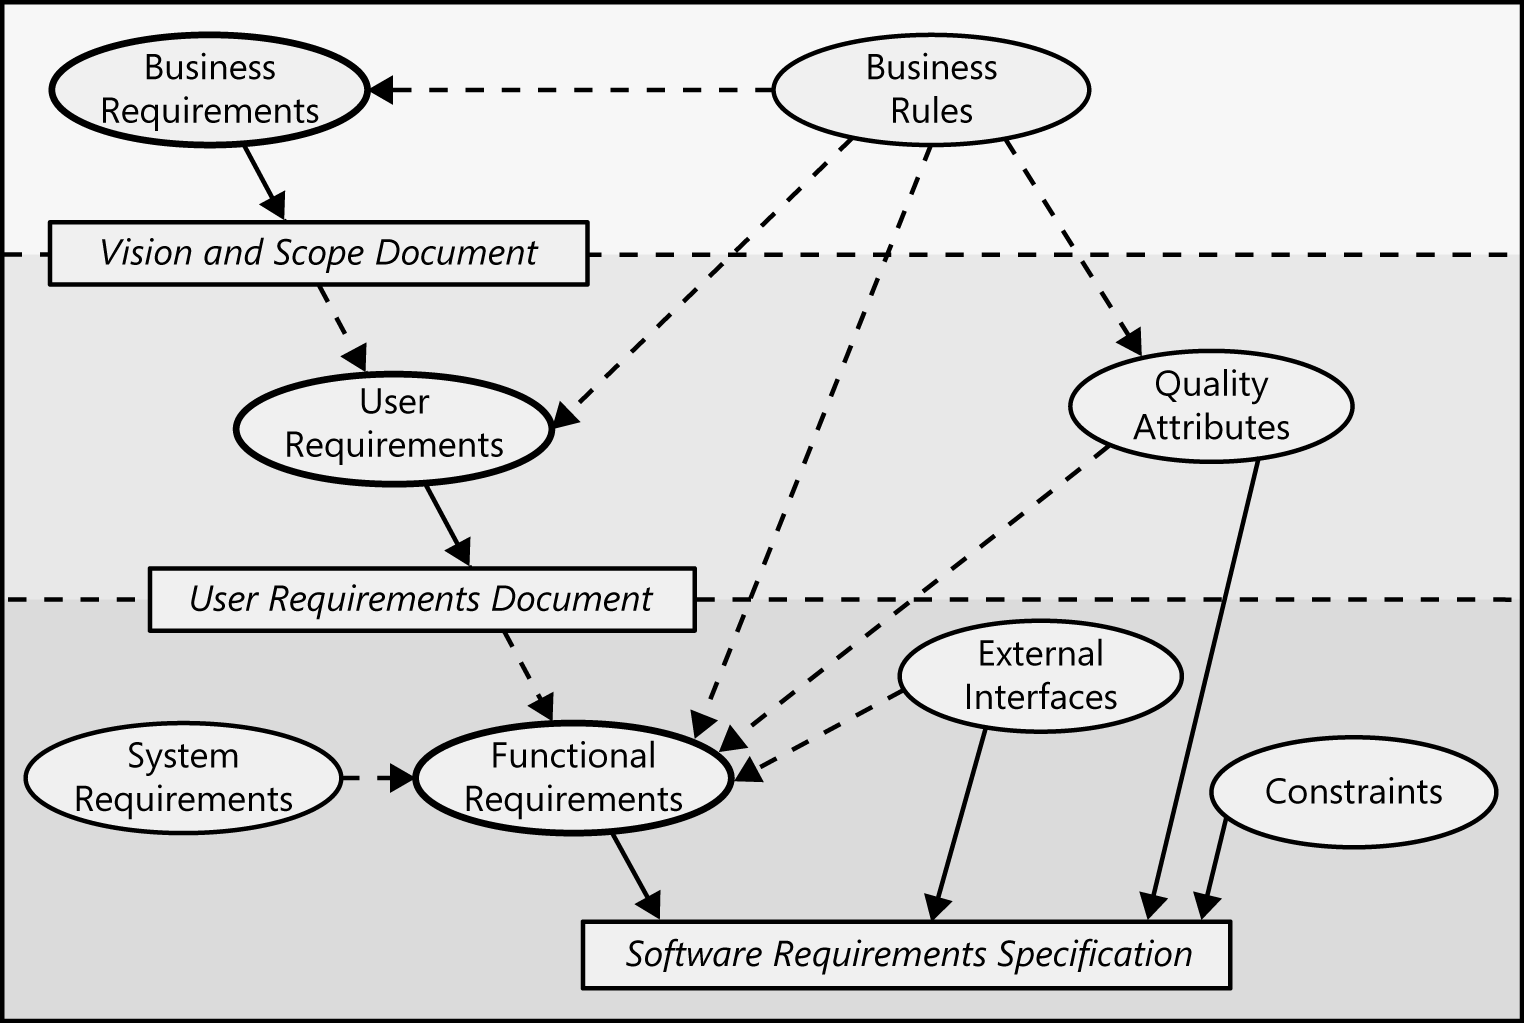
\includegraphics[width=0.75\textwidth]{TypesOfRequirements}
\centering
\caption[Types of Requirements]{Relationships among several types of requirements information~\citep[p. 8]{Wiegers2013}}
\label{fig:types_of_requirements}
\end{figure}

A \emph{feature} consists of one or more logically related system capabilities that provide value to a user and are described by a set of functional requirements. A feature can encompass multiple user requirements, each of which implies that certain functional requirements must be implemented to allow the user to perform the task described by each user requirement. %Figure~\ref{fig:feature_tree} illustrates a feature tree, an analysis model that shows how a feature can be hierarchically decomposed into a set of smaller features, which relate to specific user requirements and lead to specifying sets of functional requirements.
%
%\begin{figure}[h!]
%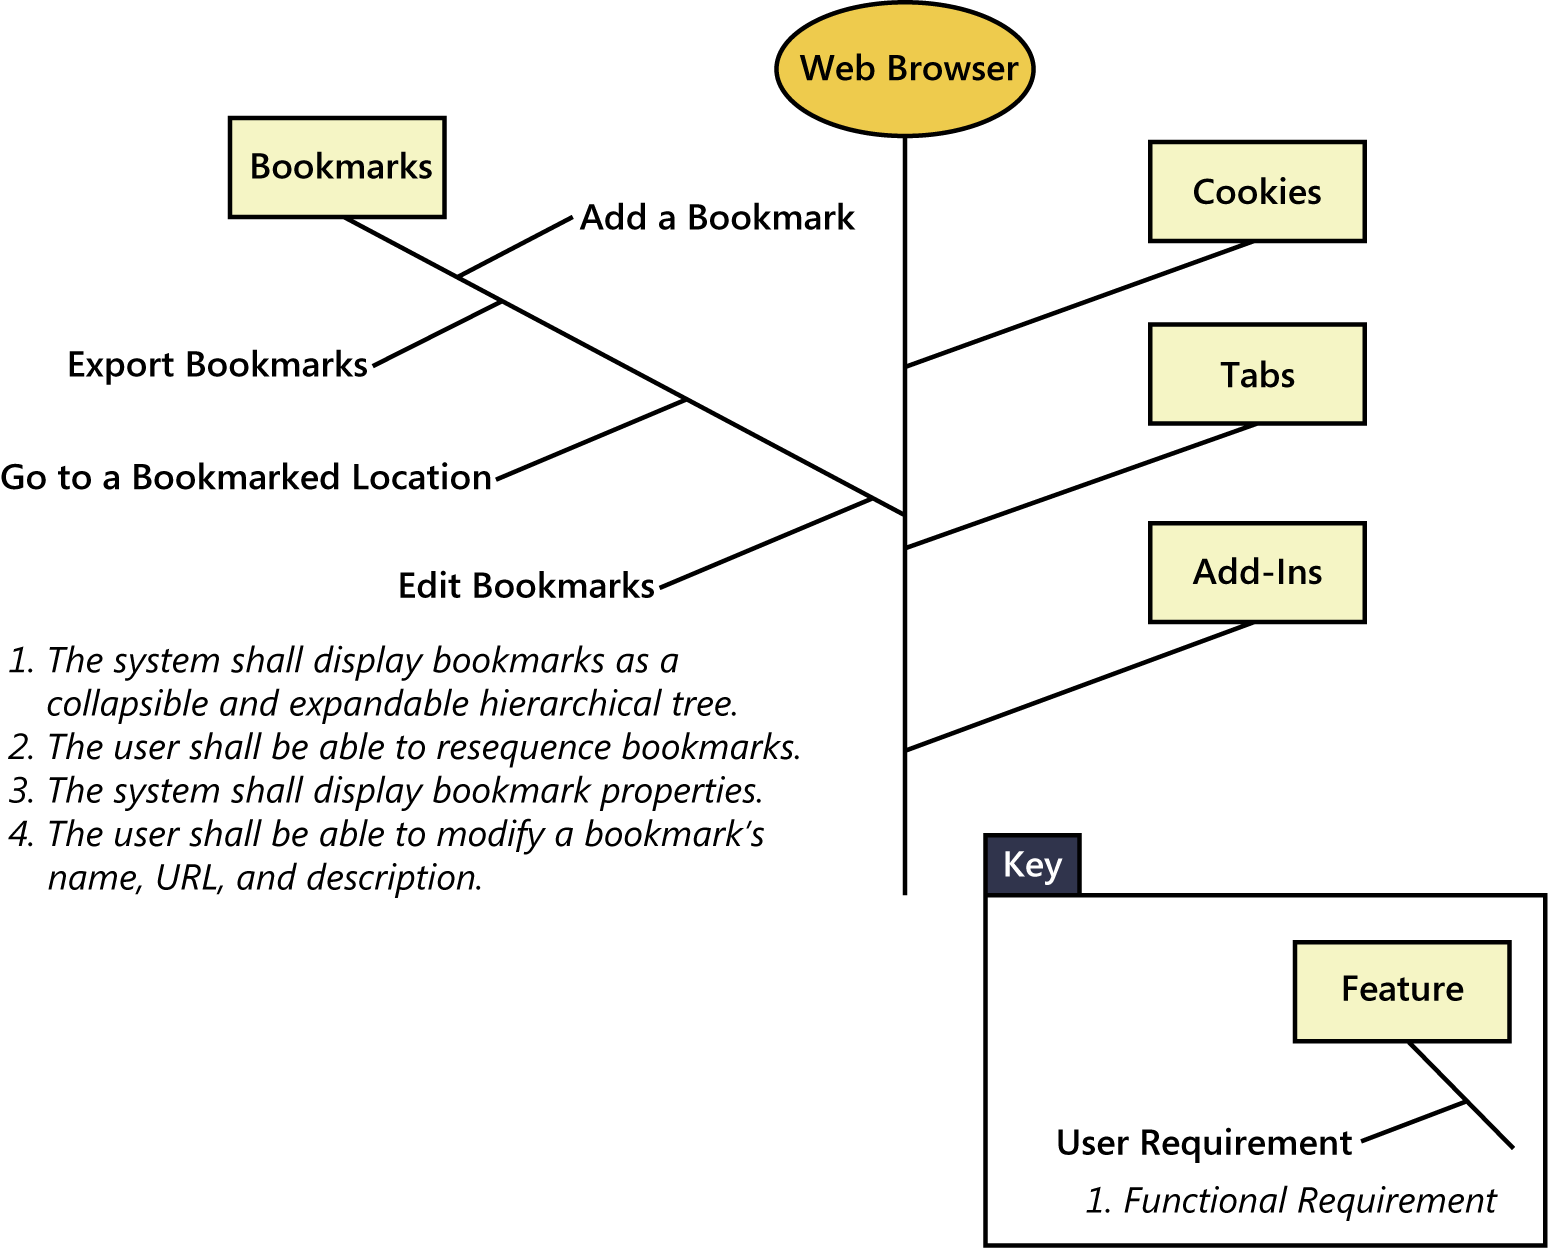
\includegraphics[width=0.75\textwidth]{FeatureTree}
%\centering
%\caption[Feature Trees]{Relationships among features, user requirements, and functional requirements~\citep[p. 11]{Wiegers2013}}
%\label{fig:feature_tree}
%\end{figure}

We have identified three major requirements deliverables: a vision and scope document, a user requirements document, and a software requirements specification. There is often no need to create three discrete requirements deliverables on each project. It often makes sense to combine some of this information, particularly on small projects. However, recognize that these three deliverables contain different information, developed at different points in the project, possibly by different people, with different purposes and target audiences~\citep{Wiegers2013}.

Requirements can also be categorised as either product or project requirements. Product requirements are those that describe properties of a software system to be built. Projects certainly do have other expectations and deliverables that are not a part of the software the team implements, but that are necessary to the successful completion of the project as a whole. These are project requirements but not product requirements. An SRS houses the product requirements, but it should not include design or implementation details (other than known constraints), project or test plans, or similar information.

\citet{Hull2011} makes an important distinction between requirements being defined in either \emph{problem} or \emph{solution} domains. In the context of requirements existing at different layers of abstraction, those at higher layers, representative of statements of need, usage modelling and stakeholder requirements, pertain to the problem domain, whereas those in lower layers, starting with system requirements, operate in the solution domain. The use of multiple levels of abstraction promotes separation of concerns and allows stakeholders, analysts and developers views to be taken in consideration. Stakeholder requirements should specify only what they want to achieve and avoid any reference to particular solutions. System requirements, on the other hand, should abstractly specify what the system will do to meet the stakeholder requirements whilst avoiding any references any particular design. Finally, subsystem and component requirements, part of architectural designs, will specify how these design meets the system requirements.


\section{Requirements Engineering}
The \emph{\citefield{SWEBOK}{maintitle}}~(\citetitle{SWEBOK}, \citeyear{SWEBOK}) identifies topics that pertain to software requirements knowledge, which concern the elicitation, analysis, specification, and validation of software requirements as well as their management during the whole life cycle of a software product.

\begin{figure}[h]
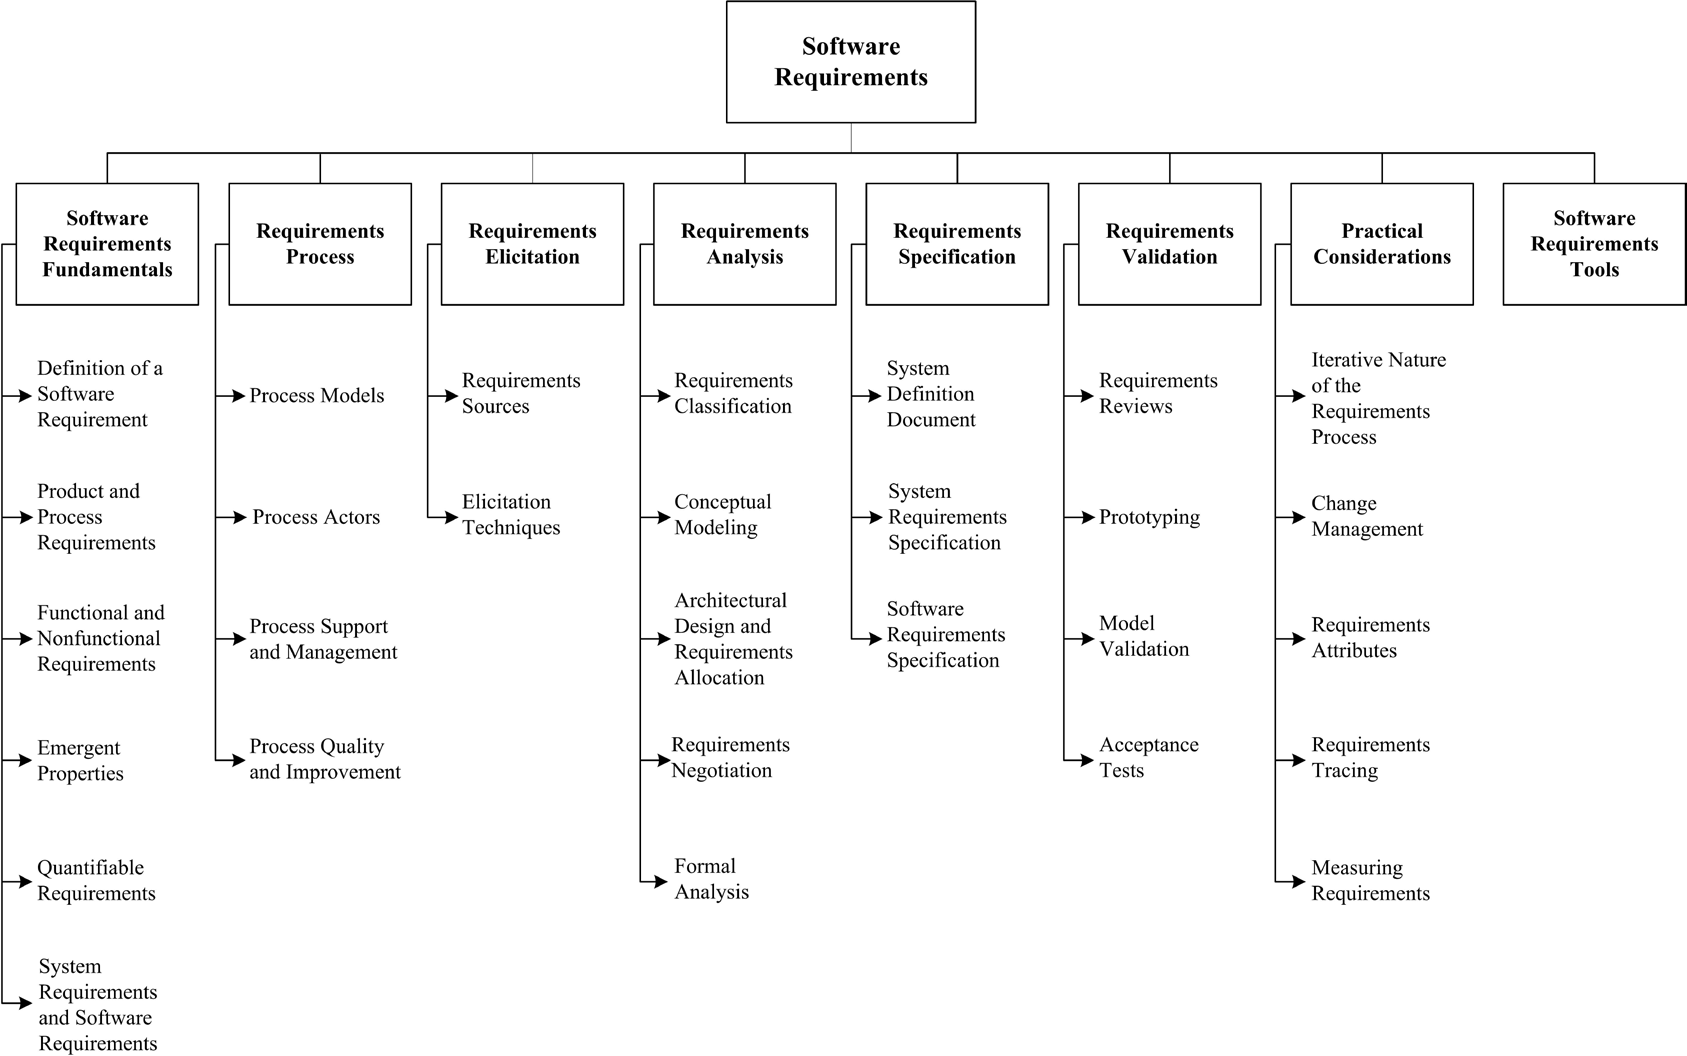
\includegraphics[width=0.75\textwidth]{swebooksoftwarerequirements}
\centering
\caption[Topics for software requirements]{Topics for the Software Requirements knowledge area~(\citetitle{SWEBOK}, \citeyear{SWEBOK})}
\label{fig:swebook_software_requirements}
\end{figure}

This section defines requirements engineering and breaks it down into its core processes and activities. We will not cover all topics contained in Figure~\ref{fig:swebook_software_requirements}, but instead focus on the more relevant ones, from the point of view of the work described in this thesis. 

The engineering aspect of requirements development and management, should not distract us from the fact that software development involves at least as much communication as it does computing, and yet we sometimes fail to appreciate that requirements engineering and, in particular, requirements elicitation -- and much of software and systems project work in general -- is primarily a human interaction challenge~\citep{Wiegers2013}. 

\subsection{Definition}
The definition in~\citefield{ieee_std_29148}{journaltitle} describes requirements engineering as an \emph{\textquote[][]{interdisciplinary function that mediates between the domains of the acquirer and supplier to establish and maintain the requirements to be met by the system, software or service of interest}}. A vital part of the systems engineering process, requirements engineering first defines the problem scope and then links all subsequent development information to it~\citep{Hull2011}. One of the most long-standing definition comes from a US Department of Defence software strategy document

\begin{displaycquote}{united1991department}
Requirements engineering involves all life-cycle activities devoted to identification of user requirements, analysis of the requirements to derive additional requirements, documentation of the requirements as a specification, and validation of the documented requirements against user needs, as well as processes that support these activities
\end{displaycquote}

A more recent definition emphasizes the goal-oriented nature of requirements engineering, and hints at the importance of understanding and documenting the relationships between requirements and other development artefacts

\begin{displaycquote}{Zave:1997:CRE:267580.267581}
Requirements engineering is the branch of software engineering concerned with the real world goals for, functions of, and constraints on software systems. It is also concerned with the relationship of these factors to precise specifications of software behaviour, and to their evolution over time and across software families
\end{displaycquote}

\citet{Hull2011} argues that both definitions omit the role that requirements play in accepting and verifying the solution. The authors propose an alternative definition

\begin{displaycquote}{Hull2011}
Requirements engineering is the subset of systems engineering concerned with discovering, developing, tracing, analysing, qualifying, communicating and managing requirements that define the system at successive levels of abstraction
\end{displaycquote}

They defend the above definition reflects better that requirements exist at multiple levels of development and also list key activities that are considered proper to requirements engineering. Similar to what we have done for the definition of requirement, it is worth breaking it down into its constituent parts. \emph{Discovering} refers to activities related to the elicitation and capture of requirements; \emph{tracing} allows setting up links to and from requirements to other artefacts; \emph{qualifying} refers to all kinds of testing activities and avoids the often confusing terms \emph{validation} -- checking formal expressions of requirements against informal needs -- and \emph{verification}, often linked with checks of requirements internal consistency within and between layers of abstraction; \emph{communicating} reflects requirements as means of communication, through which all stakeholders can agree on what is to be achieved. Finally, \emph{abstraction} makes reference to the practice of organizing requirements into layers and of tracing the satisfaction relationship between those layers.

\citet{Hull2011} makes a useful extension to software requirements that applies to complete systems -- a collection of components, machine, software and human, which co-operate in an organised way to achieve some desired result. Since components must co-operate, interfaces between components are a vital consideration in system (and requirements) engineering – interfaces between people and machine components, between machine components, and between software components.

\subsection{Processes}
Without loss of generality, we can say that requirements engineering can be split into two main processes, \emph{requirements development} and \emph{requirements management}. Requirements development can be subdivided into elicitation, analysis, specification, and validation~(\citetitle{SWEBOK},~\citeyear{SWEBOK}). Figure~\ref{fig:requirements_engineering_disciplines} below shows the domain of requirements engineering split into requirements development, encompassing the activities just mentioned, and also requirements management

\begin{figure}[h]
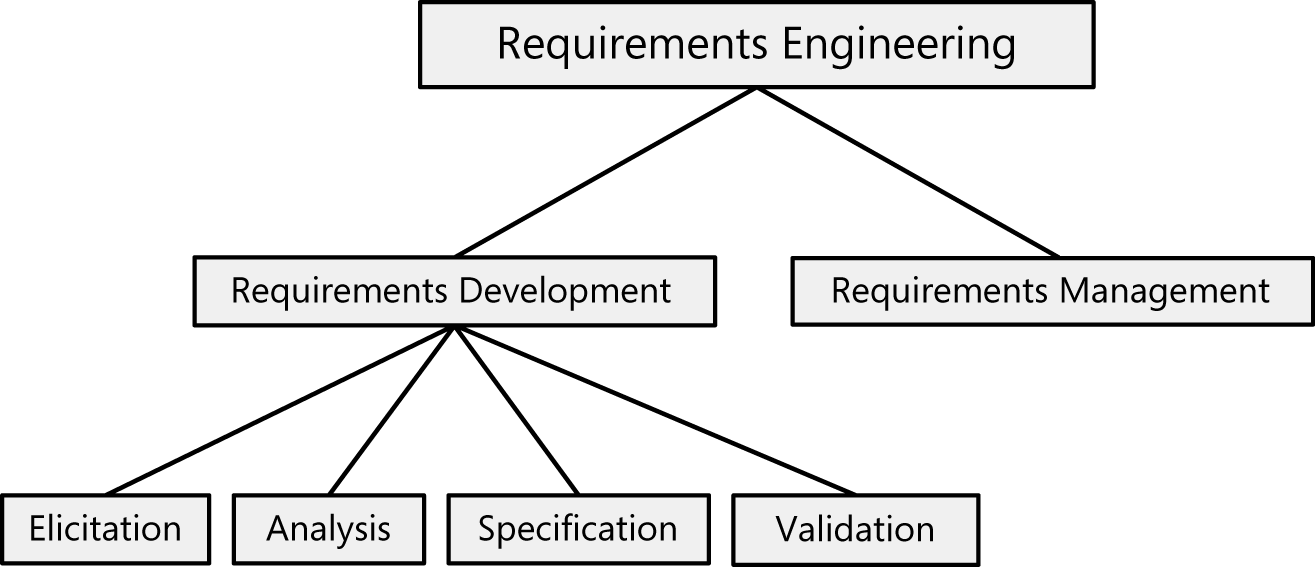
\includegraphics[width=0.75\textwidth]{RequirementsEngineeringDisciplines}
\centering
\caption[Requirements engineering disciplines]{Requirements engineering disciplines~\citep[p. 15]{Wiegers2013}}
\label{fig:requirements_engineering_disciplines}
\end{figure}

Regardless of the development life cycle followed -- be it pure waterfall, iterative, incremental, agile, or other -- these activities will be present, perhaps at different times in the project and to varying degrees of depth or detail~\citep{Wiegers2013}. Following are the essential actions in each sub-discipline:

\emph{Requirements elicitation} encompasses all of the activities involved with discovering requirements, such as interviews, workshops, document analysis and others. It is a process through which those who acquire and those who supply a given system, discover, review, articulate, understand, and document the requirements on the system and the life cycle processes~\citep{ieee_std_29148}. It typically takes either a usage-centric or a product-centric approach, although other strategies are also possible. The usage-centric strategy emphasizes understanding and exploring user goals to derive the necessary system functionality. The product-centric approach focuses on defining features that you expect will lead to marketplace or business success~\citep{Wiegers2013}.

\citefield{ieee_std_29148}{journaltitle} defines \emph{requirements analysis} as a process that traansforms stakeholder and requirement-driven views of desired services into technical views of products that could deliver those services. The main goal is to obtain a precise understanding of each requirement and representing sets of requirements in appropriate ways. This is done by distinguishing user's goals from functional requirements, determining quality expectations, business rules, suggested solutions, and other information. Through this process high-level requirements are broken down into an appropriate level of detail, the relative importance of quality attributes is assessed and requirements are allocated to software components defined in the system architecture~\citep{Wiegers2013}.

\emph{Requirements specification} involves representing and storing the collected knowledge and information in a persistent and well-organized fashion. The principal activity is translating the collected user needs into written requirements and diagrams suitable for comprehension, review, and use by their intended audiences~\citep{Wiegers2013}.

\citefield{ieee_std_29148}{journaltitle} defines \emph{requirements validation} as a confirmation by examination that requirements (individually and as a set) define the right system as intended by the stakeholders. It confirms that information gathered will enable developers to build a solution that satisfies the business objectives. The central activities are reviewing the documented requirements to correct any problems before the development group accepts them; developing acceptance tests and criteria to confirm that a product based on the requirements would meet customer needs and achieve the business objectives~\citep{Wiegers2013}.

\citet{Wiegers2013} alludes from a practical point of view, the goal of \emph{requirements development} is to accumulate a shared understanding of requirements that is good enough to allow construction of the next portion of the product -- be that 1 percent or 100 percent of the entire product -- to proceed at an acceptable level of risk. It is in line with what~\citefield{ieee_std_29148}{journaltitle} refers to as \emph{baseline} set of requirements, that is, \emph{'a specification or product that has been formally reviewed and agreed upon, that thereafter serves as the basis for further development, and that can be changed only through formal change control procedures'}. The major risk is that, if not performed properly, having to do excessive unplanned rework because of insufficient understanding of the requirements for the next chunk of work before starting design and construction~\citep{Wiegers2013}.

\citefield{ieee_std_29148}{journaltitle} identifies processes and activities within that are named differently, but that are in essence similar to the ones just described. The principal processes identified are \emph{stakeholder requirements definition} and \emph{requirements analysis} or \emph{system requirements analysis}. These two processes result in a baseline set of requirements, with a nature similar to the mentioned before. The architectural design process includes allocation and decomposition of requirements that triggers the recursive application of the requirements processes, for the definition of system element requirements and the iterative application of the requirements analysis process for derived requirements.

There is a common misconception that requirements engineering is just a single phase that is carried out and completed at the outset of product development~\citep{Hull2011}. On the contrary, requirements developed at the outset are still in use at the final stages of development. Figure~\ref{fig:testsandreqs} shows different testing activities and their relationship with requirements specified at various levels of abstraction. It is clear that stakeholder requirements are tested as part of acceptance test, a late stage in any software development method, be it traditional or agile. In addition, each testing activity has a separate concern, with acceptance test focusing on validating the product; system test verifying the system and integration and component testing, verifying subsystem and components requirements, respectively.
\begin{figure}[h]
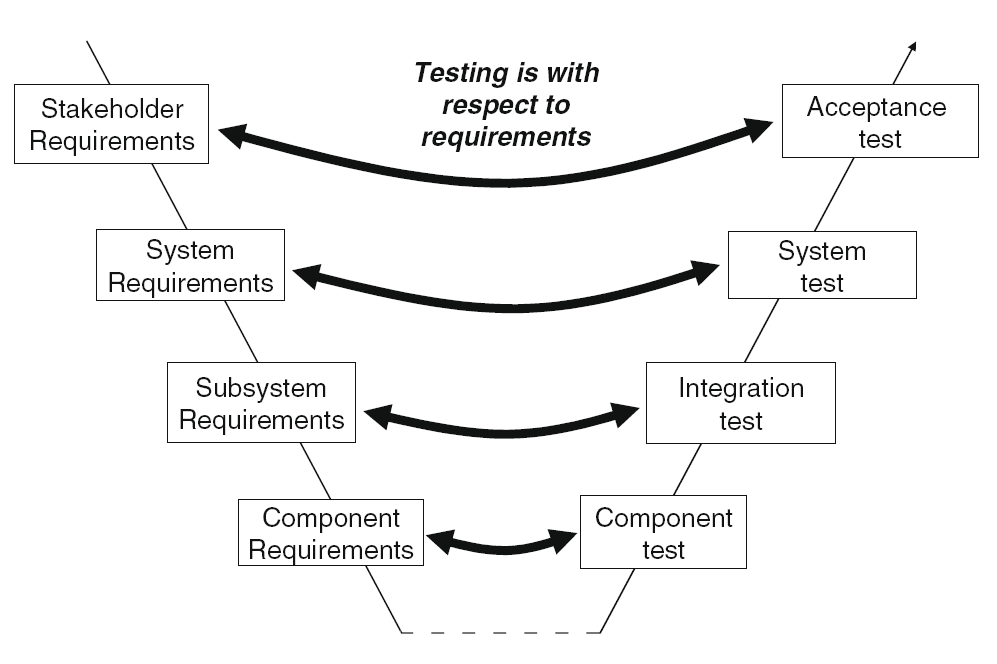
\includegraphics[width=0.75\textwidth]{RoleOfRequirementsInRelationToTesting}
\centering
\caption{Testing activities and requirements}
\label{fig:testsandreqs}
\end{figure}

If requirements are to play such a central role in systems development, they need to be maintained. Hence requirements engineering connects strongly with change management. Independently of where new or changed requirements come from, the impact of that change on quality, cost and schedule needs to be assessed. This assessment informs decisions to either accept or reject a change; negotiate the cost of change and organise and assign work to development teams~\citep{Hull2011}. The purpose of \emph{requirements management} is to anticipate and accommodate the very real changes that you can always expect so as to minimize their disruptive impact on the project. Core requirements management activities include defining the requirements baseline; evaluating the impact of proposed requirements changes; establishing any relationships and dependencies between requirements and tracking requirements status and change activity throughout the project~\citep{Wiegers2013}.

The key concept that enables this kind of impact analysis is requirements tracing, primarily concerned with understanding how high-level requirements -- objectives, goals, aims, aspirations, expectations, needs -- are turned into low-level requirements. It is therefore primarily concerned with the relationships between layers of information. For example, in a business context the concern is how a business vision determines a set of objectives and how these may be implemented as changes to the organisation and processes. In a systems development context, the focus is in determining how stakeholder requirements are met by system requirements and their breakdown in subsystems and components. Requirements tracing allow measuring the impact of change, track progress against a set of requirements and assess benefit against cost of implementation~\citep{Hull2011}.

\section{Agile Requirements Engineering}
\subsection{Agile development}
Traditional software development methods advocate a simple top-down flow of requirements information. In agile development approaches we expect cycles and iteration among the business, user, and functional requirements. An effective change process that includes impact analysis ensures that the right people make informed business decisions about which changes to accept and that the associated costs in time, resources, or feature trade-offs are addressed~\citep{Wiegers2013}.

Often, it's impossible or unnecessary to fully specify the functional requirements before commencing design and implementation. In those cases, you can take an iterative or incremental approach, implementing one portion of the requirements at a time and obtaining customer feedback before moving on to the next cycle. This is the essence of agile development, learning just enough about requirements to do thoughtful prioritization and release planning so the team can begin delivering valuable software as quickly as possible. This isn't an excuse to write code before contemplating requirements for that next increment, though. Iterating on code is more expensive than iterating on concepts~\citep{Wiegers2013}.

\subsection{Practices}

In agile approaches handling of non-functional requirements is ill defined. Customers or users talking about what they want the system to do normally do not think about resources, maintainability, portability, safety or performance~\cite{Paetsch:2003tl}.

\subsection{Behaviour driven development~(BDD)}
\label{ch:Background:sec:bdd}
\citet{Hull2011} advocates the use of modelling techniques as a mechanism of fostering understanding and communication of ideas associated with system development. A good model is one which is easily communicated. They need to be used for communication within a development team, and also to an organisation as a whole including the stakeholders. The uses of a model can be diverse and cover a wide
spectrum. It might be to model the activities of an entire organisation or to model a specific functional requirement of a system. It this latter use that is at the core of Behaviour Driven Development (BDD).

\citet{North2006} first described BDD in a blog post 

\begin{figure}[h]
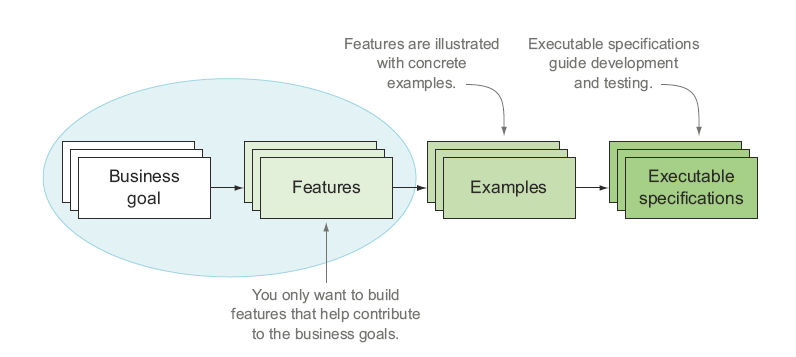
\includegraphics[width=0.75\textwidth]{BDD}
\centering
\caption{BDD: From business goals to executable specifications}
\label{fig:bdd_from_goals_to_specs}
\end{figure}

\chapter{On non-functional requirements}
\label{ch:Background:sec:nfr_research}
For many years, the requirements for a software product have been classified broadly as either functional or non-functional. The functional requirements are evident: they describe the observable behaviour of the system under various conditions. However, many people dislike the term 'non-functional'. That adjective says what the requirements are not, but it doesn't say what they are. We are sympathetic to the problem, but we lack a perfect solution~\citep{Wiegers2013}.

Other-than-functional requirements might specify not what the system does, but rather how well it does those things. They could describe important characteristics or properties of the system. These include the system's availability, usability, security, performance, and many other characteristics. Some people consider non-functional requirements to be synonymous with quality attributes, but that is overly restrictive. For example, design and implementation constraints are also non-functional requirements, as are external interface requirements~\citep{Wiegers2013}.

Still other non-functional requirements address the environment in which the system operates, such as platform, portability, compatibility, and constraints. Many products are also affected by compliance, regulatory, and certification requirements. There could be localization requirements for products that must take into account the cultures, languages, laws, currencies, terminology, spelling, and other characteristics of users. Though such requirements are specified in non-functional terms, the business analyst typically will derive numerous bits of functionality to ensure that the system possesses all the desired behaviours and properties~\citep{Wiegers2013}.

In this thesis, rather than worry about precisely what to call these sorts of information, best practice is to ensure that they are part of requirements elicitation and analysis activities. A product can be delivered with all the desired functionality but that users hate because it doesn't match their (often unstated) quality expectations~\citep{Wiegers2013}.


\section{Product or process oriented approaches}

\section{Requirements as Goals}
\label{ch:gore}
The use of goals in requirements engine has received increasing attention over the past few years. Such recognition has led to a whole stream of research on goal modelling, goal specification, and goal-based reasoning for multiple purposes, such as requirements elaboration, verification or conflict management, and under multiple forms, from informal to qualitative to formal~\citep{Lamsweerde:2001wpba}.

In addition, the requirements engineer needs to explore alternatives and evaluate their feasibility and desirability with respect to business goals. We share the view that goal-oriented analysis complements and strengthens traditional requirements engineering techniques by offering a means for capturing and evaluating alternative ways of meeting business goals~\citep{MylopoulosExpl2001}.

\section{Goal oriented requirements language~(GRL)}
Goals denote the objectives a system must meet. Eliciting high level goals early in the development process is crucial. However, goal-oriented requirements elicitation [15] is an activity that continues as development proceeds, as high-level goals (such as business goals) are refined into lower-level goals (such as technical goals that are eventually operationalised in a system). Eliciting goals focuses the requirements engineer on the problem domain and the needs of the stakeholders, rather than on possible solutions to those problems\citep{Nuseibeh:2000ub}.

A goal is an objective the system under consideration should achieve. Goals capture, at different levels of abstraction, the various objectives the system under consideration should achieve~\citep{Lamsweerde:2001wpba}. Goals also cover different types of concerns: functional concerns associated with the services to be provided, and non-functional ones, associated with quality of service, such as safety, security, accuracy, performance, and so forth.

\pagebreak

\chapter{Extending behaviour-driven development}
\label{ch:Extendingbdd}

\begin{itemize}
\item Compare with Advanced Traceability in~\citep{Hull2011}
\end{itemize}


\chapter{Conclusion}
\label{ch:Conclusion}
Out work helps to address some of the most common requirements risks~\citep[p. 20]{Wiegers2013}.
\begin{itemize}
\item Insufficient user involvement
\item Inaccurate planning
\item Creeping user requirements
\item Ambiguous requirements
\item Gold plating
\item Overlooked stakeholders
\end{itemize}
\appendix
Our work is also actual and contributes to major requirements trends in recent in the past decade, including
\begin{itemize}
\item The recognition of business analysis as a professional discipline
\item The maturing of tools both for managing requirements in a database and for assisting with requirements development activities such as prototyping, modelling, and simulation
\item The increased use of agile development methods and the evolution of techniques for handling requirements on agile projects
\item The increased use of visual models to represent requirements knowledge
\end{itemize}

Writing the requirements isn't the hard part. The hard part is determining the requirements. Writing requirements is a matter of clarifying, elaborating, and recording what you've learned. A solid understanding of a product's requirements ensures that your team works on the right problem and devises the best solution to that problem. Without knowing the requirements, you can't tell when the project is done, determine whether it has met its goals, or make trade-off decisions when scope adjustments are necessary. It can cost far more to correct a defect that's found late in the project than to fix it shortly after its creation. Shortcomings in requirements practices pose many risks to project success, where success means delivering a product that satisfies the user's functional and quality expectations at the agreed-upon cost and schedule~\citep{Wiegers2013}.

Some of the most common requirements risks are insufficient user involvement; inaccurate planning; creeping user requirements ; ambiguous requirements and overlooked stakeholders. Sound requirements processes emphasize a collaborative approach to product development that involves stakeholders in a partnership throughout the project. Eliciting requirements lets the development team better understand its user community or market, a critical success factor. Emphasizing user tasks instead of superficially attractive features helps the team avoid writing code that no one will ever execute. Customer involvement reduces the expectation gap between what the customer really needs and what the developer delivers. Documented and clear requirements greatly facilitate system testing. All of these increase your chances of delivering high-quality products that satisfy all stakeholders~\citep{Wiegers2013}.

\chapter{Typical chapter contents}\fxnote{Remove}


\underline{Start of chapter}
\paragraph{General advice}
Link back to previous parts in particular previous chapter\\
State the aim of the chapter\\
Outline how you intend to achieve this aim in the form of an overview of contents\\

\noindent\underline{Contents}
\paragraph{Discussion or Analysis}
\begin{itemize}
\item What's important
\item What overall themes can be identified
\item What can be observed or learned
\item What limitations or shortcomings have been identified
\item Situate the chapter within the whole thesis
\end{itemize}
\paragraph{Summary}
\begin{itemize}
\item Replies to the introduction by briefly identifying the chapter's achievements and sets the scene for the next chapter
\end{itemize}

\noindent\underline{End of chapter}
\paragraph{General advice}
Start with a strong summary of the main findings of this chapter with academic references and relate it with current theory.\\
Relates this chapter results to earlier analysis.\\
End with a strong lead into next chapter.\\

\printbibliography

\end{document}
